\chapter{Progettazione del sistema}

\section{Strumenti e Metodologie Utilizzate}

Dovendo progettare un \textbf{applicativo a interfaccia grafica} appoggiato su un \textbf{database}, 
si è deciso di rifarsi al \textbf{pattern architetturale EBC} (\textbf{Entity-Boundary-Control}) per
la progettazione del sistema. Tale pattern è stato scelto in quanto accentua 
\textbf{la separazione} tra le varie componenti del sistema, rendendo
più \textbf{semplice la manutenzione e l'aggiornamento} del sistema stesso.

Per la realizzazione dell'interfaccia grafica, si è scelto di utilizzare il 
\textbf{framework JavaFX}, con l'aiuto della libreria \textbf{MaterialFX} 
per alcuni componenti e del software \textbf{SceneBuilder} per creare lo scheletro
delle schermate, in quanto è il framework più moderno disponibile 
per tale scopo e \textbf{consigliato da Oracle}.

Per la realizzazione dell'interazione dell'applicativo col database, preesistente 
alla progettazione e creato in \textbf{PostgreSQL}, si è scelto di utilizzare
\textbf{JDBC}, in quanto è il metodo più semplice e diretto per interagire con un
database in Java.

Inoltre, per la gestione di dipendenze e routine di progetto, si è utilizzato
\textbf{Maven}, in quanto è il gestore di progetti più diffuso e consigliato per
progetti Java.

\begin{note}[Teamwork e Versionamento]
  Per la gestione del progetto in team, si è deciso di utilizzare \textbf{Git} come
  sistema di versionamento, con \textbf{GitHub} come piattaforma di hosting. Lo sviluppo è
  avvenuto su \textbf{branch separati} e \textbf{merge request} per la \textbf{code review}.
  Inoltre, si è deciso di utilizzare \textbf{GitHub Actions} per il controllo della qualità
  del codice. Maggiori informazioni su come è stato gestito il progetto sono disponibili
  nel README del \exlink{https://github.com/RiccardoElena/UninaDelivery/tree/master}{repository del progetto}.
\end{note}

\section{Architettura del Sistema e Class Diagram}

Il sistema è stato progettato seguendo il pattern architetturale EBC, che prevede
la suddivisione del sistema in tre componenti principali: \textbf{Entity}, \textbf{Boundary}
e \textbf{Control}.

\begin{note}[Leggibilità dei Class Diagram]
  Essendo il \textbf{Class Diagram} particolarmente denso, si è scelto di presentare
  prima i \textbf{Class Diagram} di ogni package singolarmente per approfondire
  \textbf{metodi e attributi} delle classi oltre che le \textbf{relazioni} tra esse 
  all'interno del singolo componente, per poi presentare il \textbf{Class Diagram}
  completo del sistema per avere una visione d'insieme sulle interazioni tra le
  varie componenti.

  Per migliorare la leggibilità, si è scelto di utilizzare \textbf{colori} per
  evidenziare l'appartenenza di una classe a un package e di utilizzare.
\end{note}

\subsection{Entity}

La componente \textbf{Entity} è la componente che si occupa di gestire i dati del sistema.
In particolare, si occupa di gestire la \textbf{mappatura} dei dati del sistema, ovvero
la conversione dei dati presenti nel database in oggetti Java e viceversa.

Per la gestione di tale componente, si è deciso creare due \textbf{package}, il primo
contenente le classi che implementano il \textbf{design pattern DAO}
(\textbf{Data Access Object}), ovvero le uniche classi a potersi occupare dell'interazione
col database e della mappatura dei dati, e il secondo contenente le classi che implementano il
\textbf{design pattern DTO} (\textbf{Data Transfer Object}), ovvero le classi che
rappresentano il modello di dominio, ovvero gli oggetti mappati.

In particolare, le classi \textbf{DAO} implementano le operazioni di \textbf{CRUD} (\textbf{Create, Read, Update, Delete})
sui dati del database, mentre le classi \textbf{DTO} implementano metodi \textbf{getter} e \textbf{setter}
per i dati mappati oltre che a minima logica relativa allo specifico oggetto.

Inoltre, per enfatizzare la manutenibilità e l'estensibilità del sistema, il package 
\textbf{DAO} utilizza un'interfaccia generica \textbf{BaseDAO} che implementa le operazioni
fondamentali di \textbf{CRUD}, delle interfacce specifiche per ogni classe \textbf{DTO} 
che estendono \textbf{BaseDAO} contenenti le operazioni specifiche per ogni classe \textbf{DTO}
e, infine, una classe per ognuna di queste interfacce specifica per il \textbf{DBMS} scelto.

Questo approccio permette di \textbf{separare} la logica d'interazione col database dalla
logica di gestione dei dati, permettendo di \textbf{cambiare} il \textbf{DBMS} senza dover
modificare la logica di gestione dei dati e di \textbf{aggiungere} nuove classi \textbf{DTO}.

Infine, il package \textbf{DAO} contiene anche una classe \textbf{DBConnection} che
implementa il \textbf{design pattern Singleton} e si occupa di gestire la connessione
al database, permettendo di avere una sola connessione aperta per l'intera esecuzione
dell'applicativo.

\newpage
\begin{figure}[H]
  \centering
  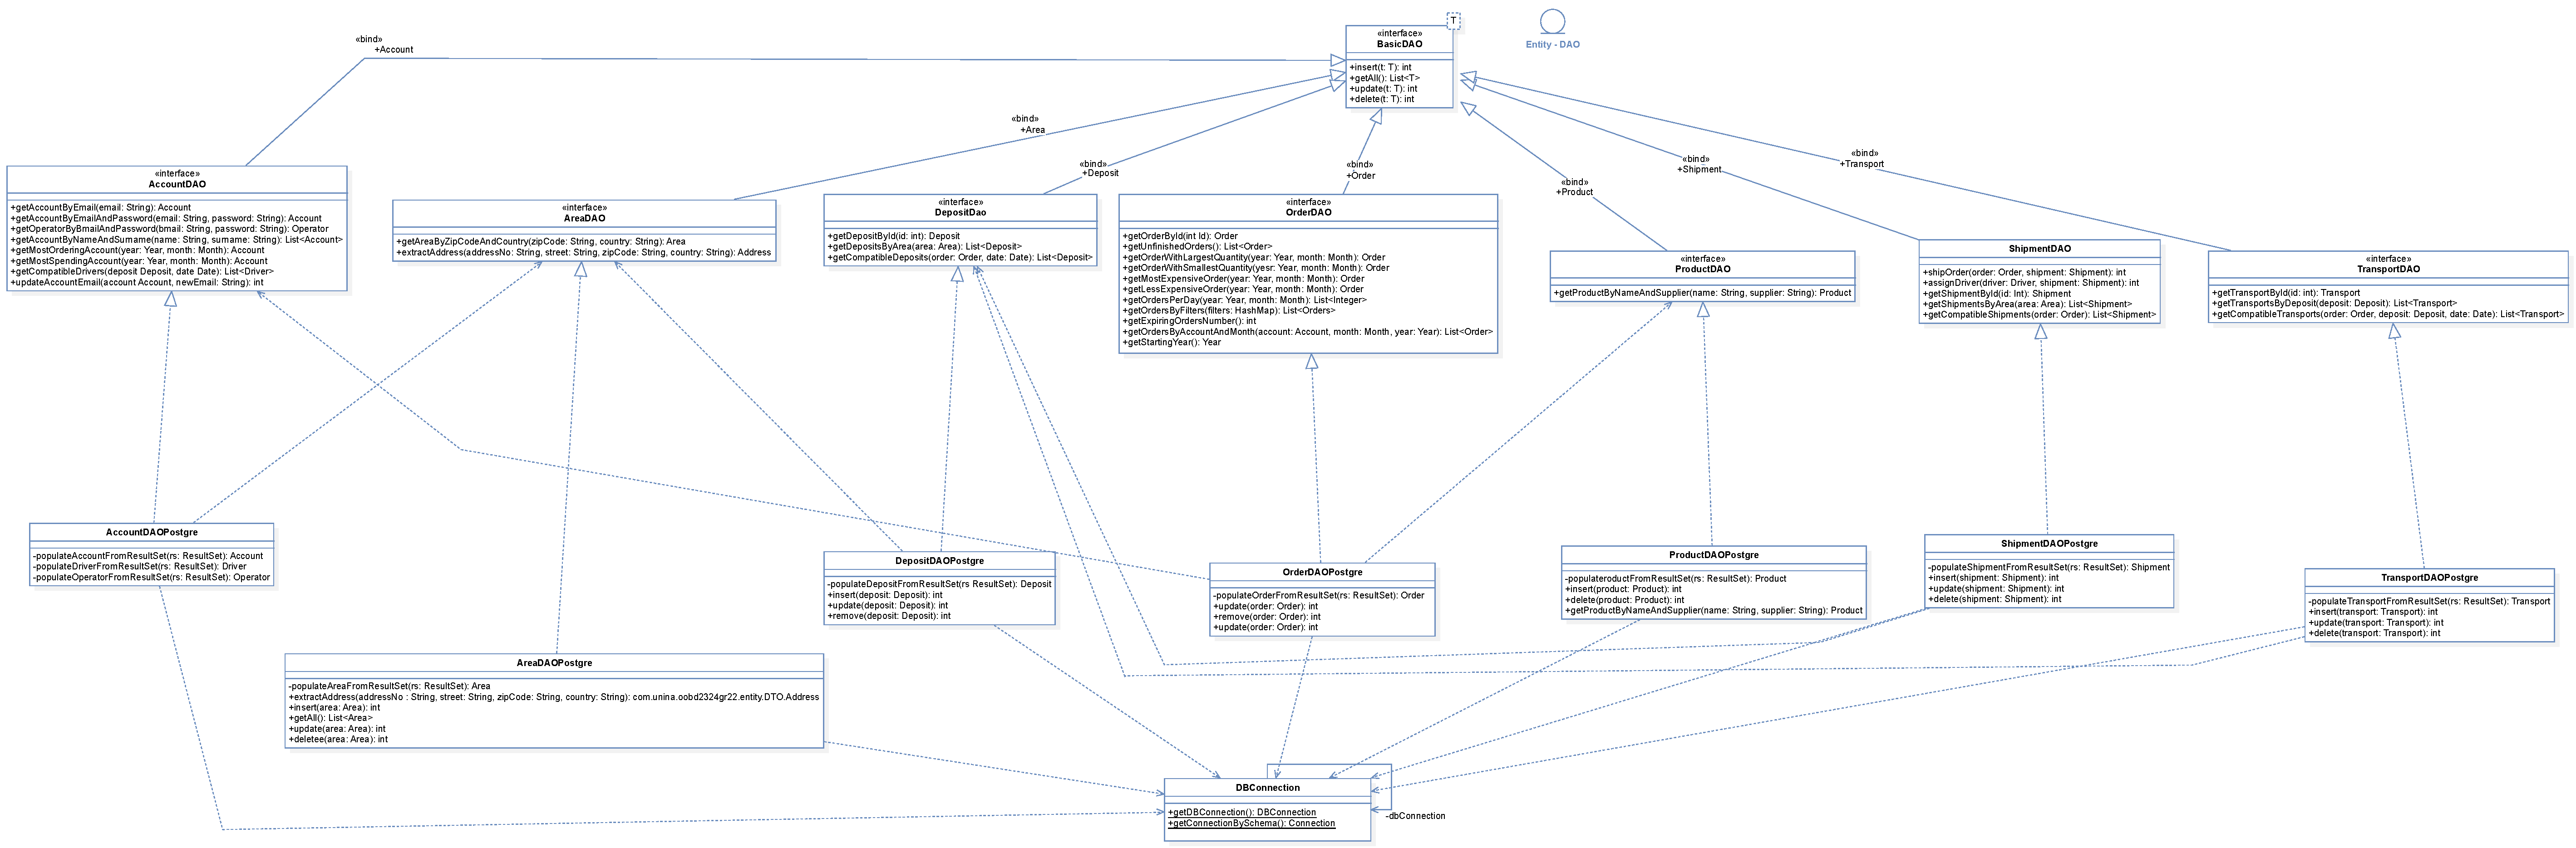
\includegraphics[width=\textwidth]{classDiagrams/dao}
  \caption{Class Diagram del package Entity/DAO}
\end{figure}

\begin{figure}
  \centering
  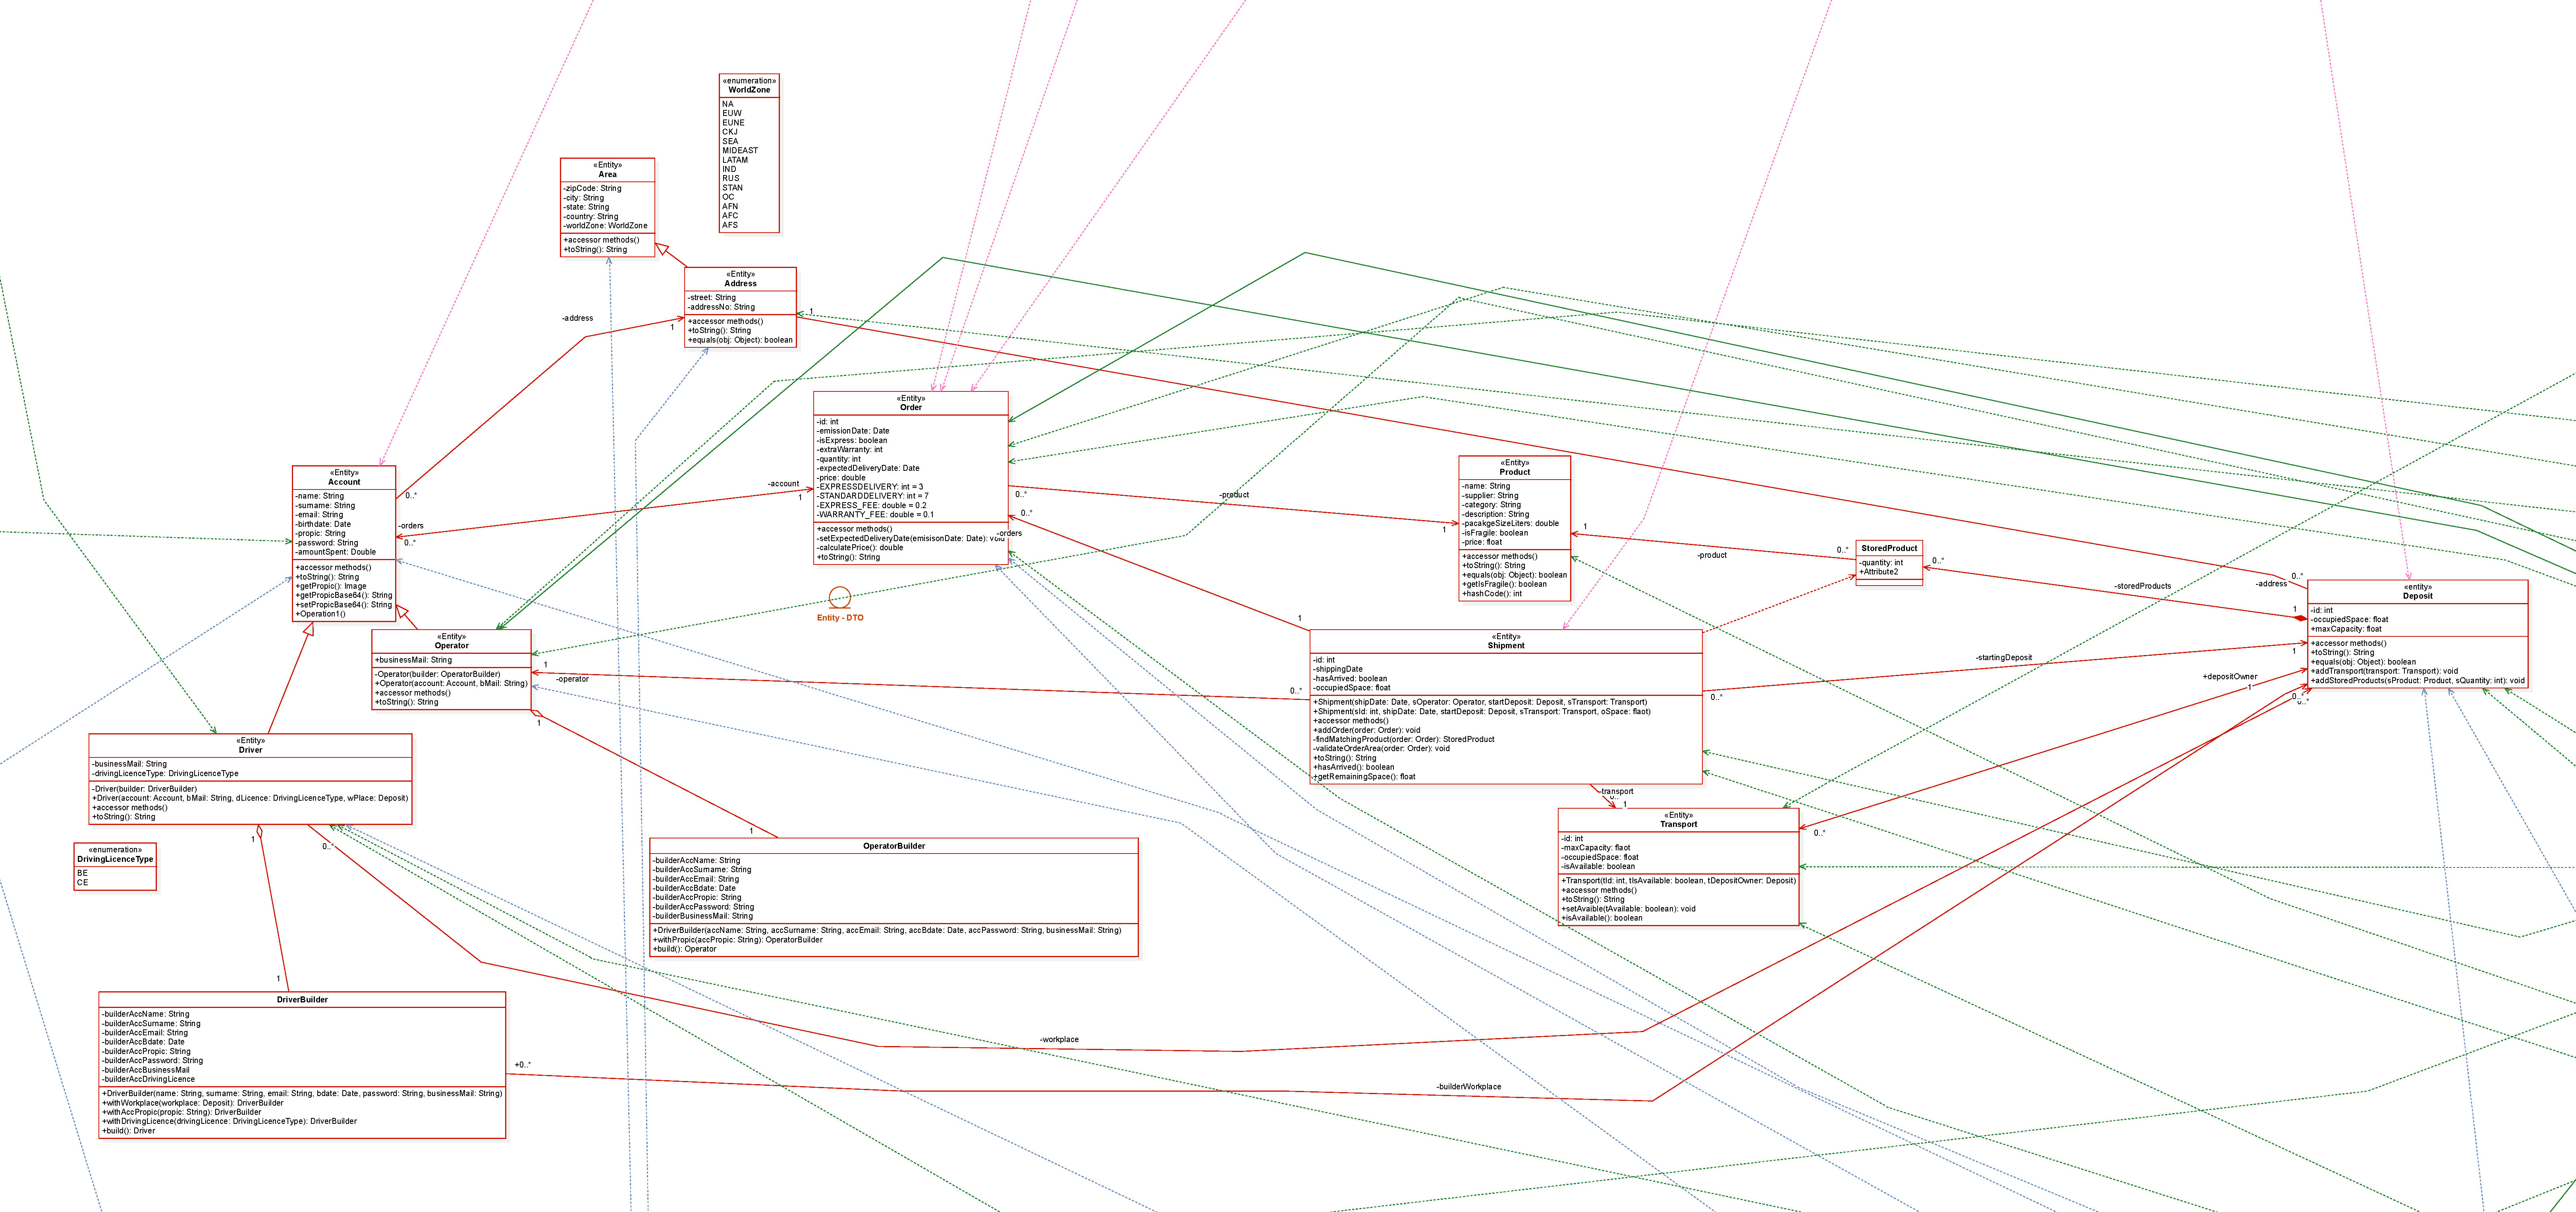
\includegraphics[width=\textwidth]{classDiagrams/dto}
  \caption{Class Diagram del package Entity/DTO}
\end{figure}

\newpage

\subsection{Boundary}

La componente \textbf{Boundary} è la componente che si occupa di gestire l'interfaccia,
ovvero la parte visuale
 del sistema. Essendo che \textbf{JavaFX} permette di gestire
la struttura delle pagine utilizzando file \textbf{FXML} e il suo stile utilizzando fogli
\textbf{CSS}, questa componente si occupa di gestire la logica di visualizzazione
 e d'interazione con l'utente.

In particolare, le classi \textbf{Boundary} implementano gli \textbf{EventListner} per i vari
componenti grafici, ovvero i metodi che vengono chiamati quando l'utente interagisce, 
oltre che l'eventuale \textbf{logica di visualizzazione condizionata} di alcuni componenti 
delle pagine dipendente da \textbf{interazione dell'utente} o da dati forniti da 
\textbf{livelli sottostanti dell'architettura}.

Inoltre, per enfatizzare la manutenibilità e l'estensibilità del sistema, oltre che la pulizia
del codice seguendo il principio \textbf{DRY} (\textbf{Don't Repeat Yourself}), si è 
deciso di generalizzare le operazioni comuni a più pagine in classi astratte, che
vengono estese dalle classi concrete per ogni pagina.

Ciò snellisce il codice della singola pagina, permette di avere uniformità stilistica 
e implementativa per le pagine, di \textbf{cambiare} la \textbf{struttura}
della pagina senza dover modificare la logica di visualizzazione e di \textbf{aggiungere} nuove
pagine senza dover riscrivere la logica comune.

\begin{figure}[H]
  \centering
  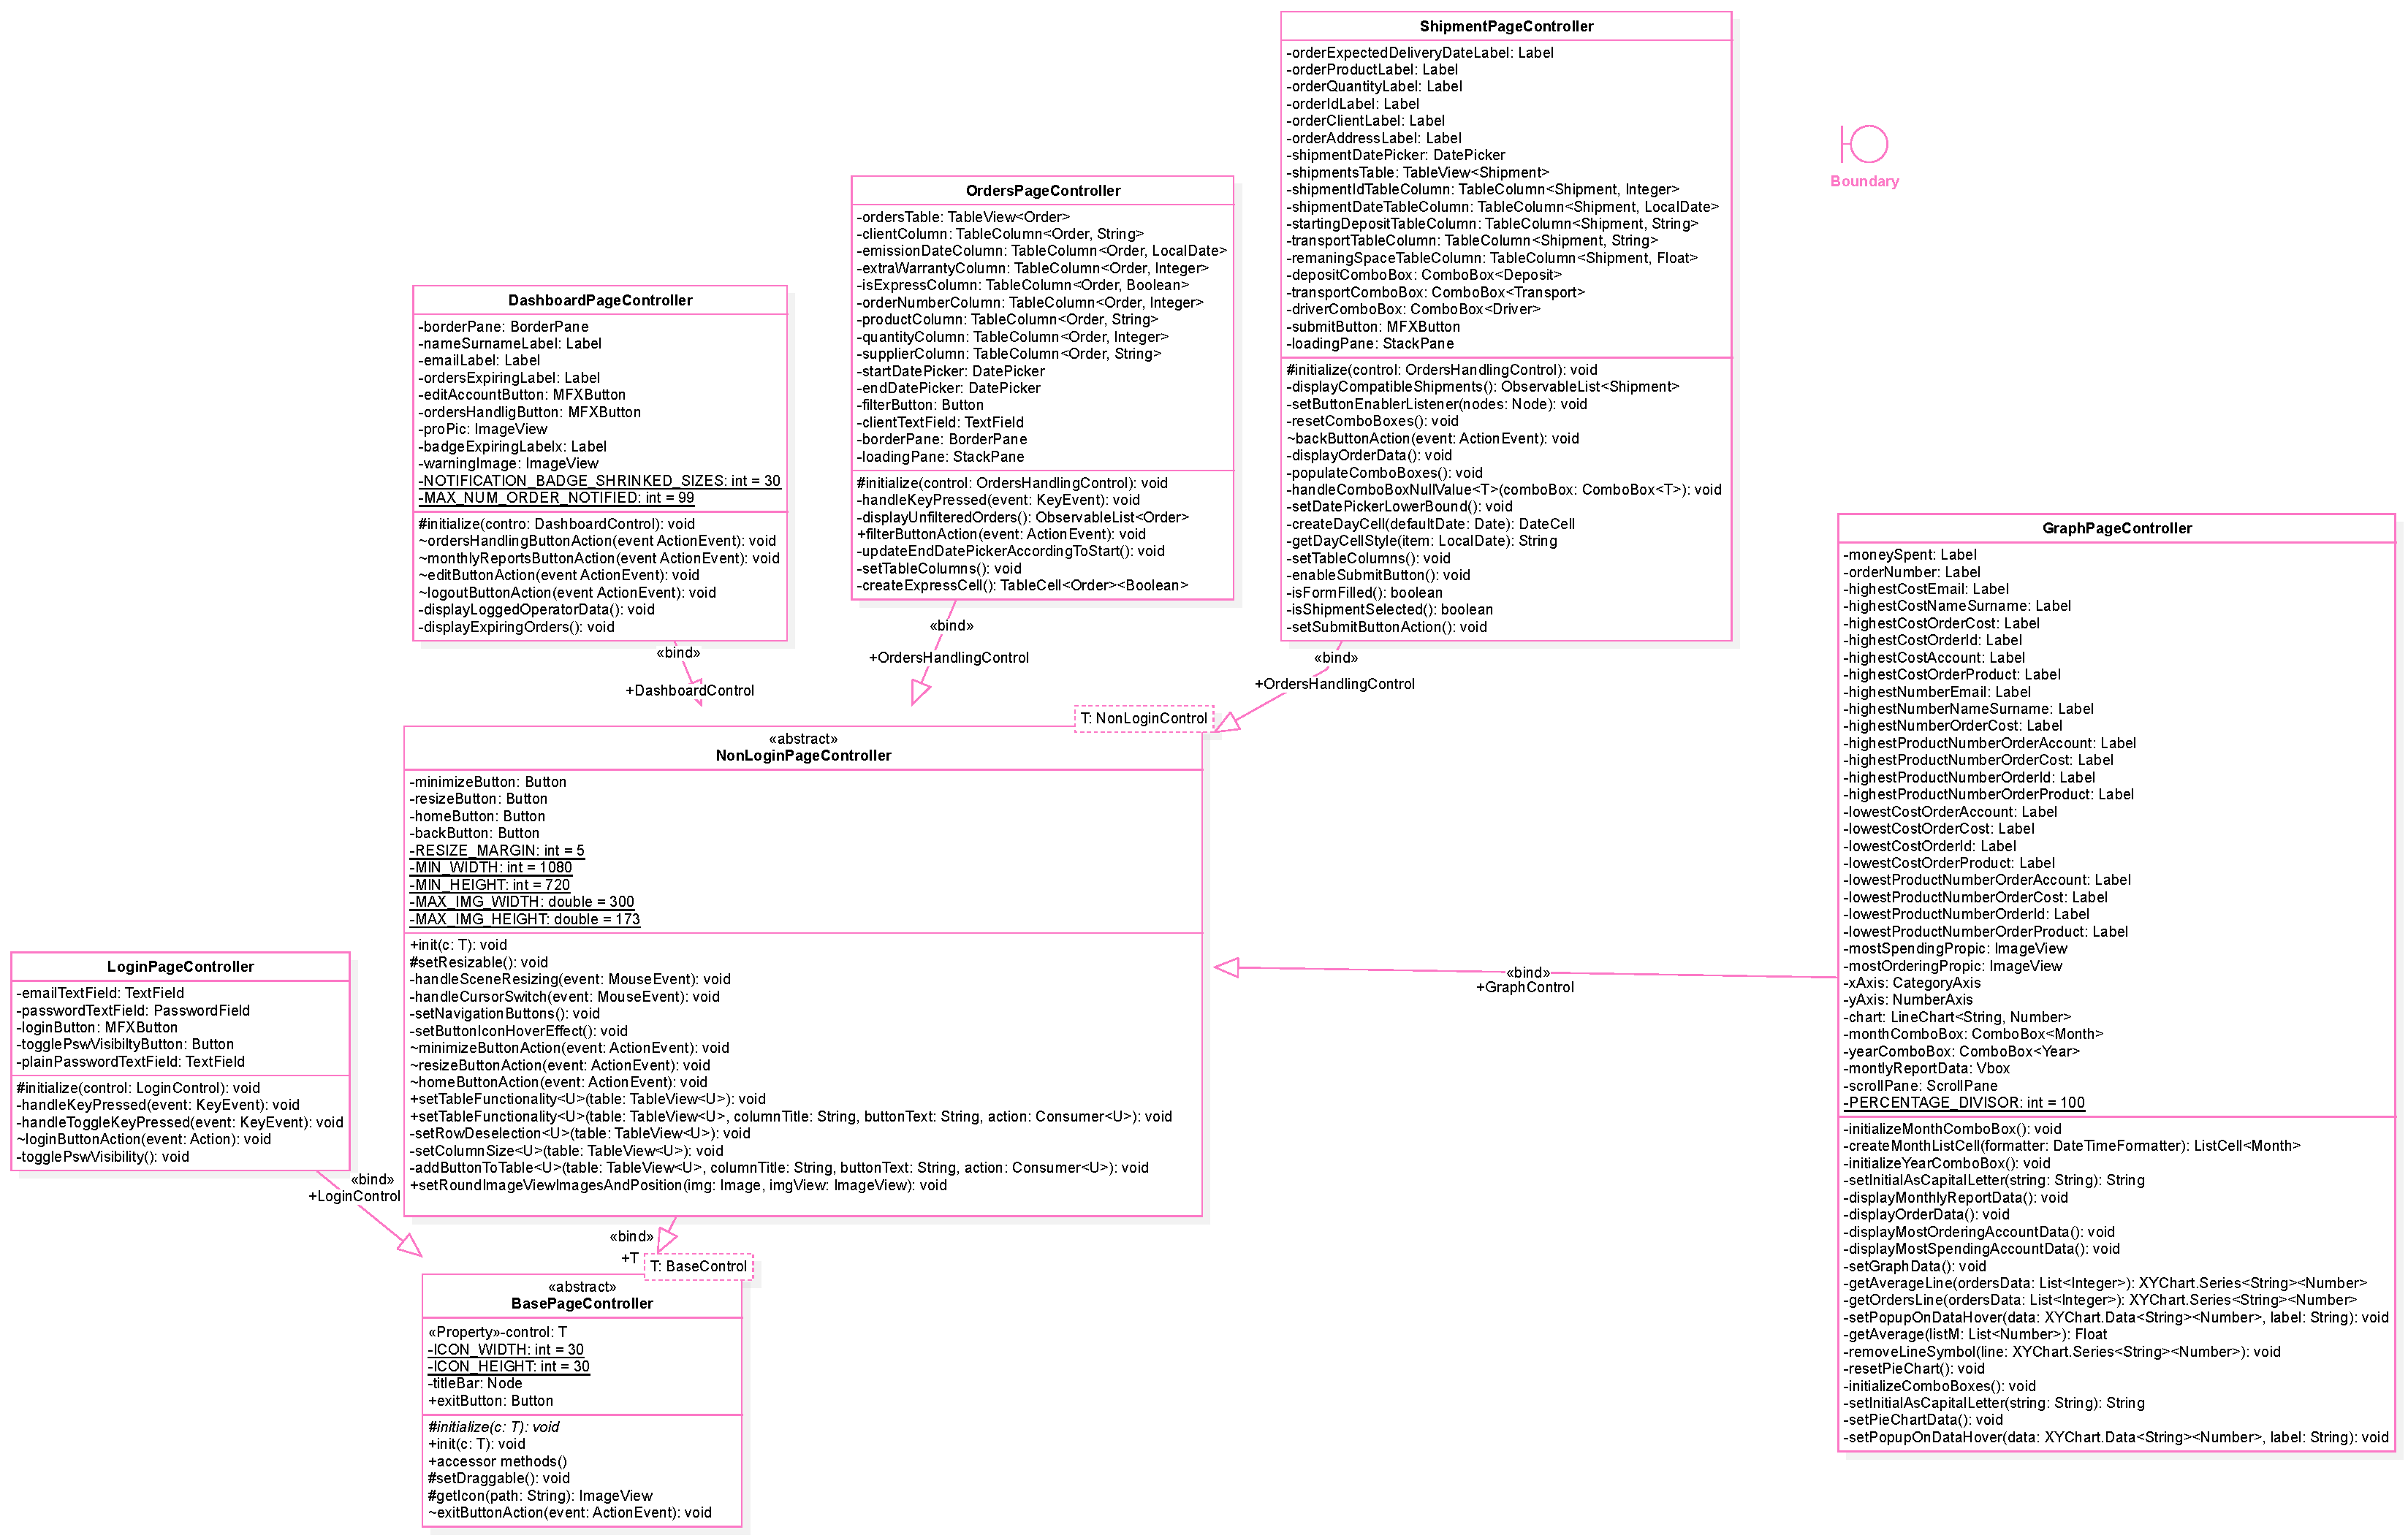
\includegraphics[width=\textwidth]{classDiagrams/boundaries}
  \caption{Class Diagram del package Boundary}
\end{figure}

\newpage

\subsection{Control}

La componente \textbf{Control} è la componente che si occupa di gestire la \textbf{logica di
business} del sistema, ovvero la logica che si occupa di gestire i dati e le operazioni
su di essi, oltre che mettere in comunicazione le altre due componenti.

In particolare, le classi \textbf{Control}, una per \textbf{funzionalità} (\textbf{use case}),
implementano la logica di \textbf{validazione} dei dati inseriti dall'utente, 
la logica di \textbf{gestione} dei dati, ovvero la logica di \textbf{CRUD} e 
la logica di \textbf{comunicazione} con le altre componenti.

Come per le altre componenti, per enfatizzare la manutenibilità e l'estensibilità del sistema,
si è deciso di generalizzare le operazioni comuni a più classi in classi astratte, che
vengono estese dalle classi concrete per ogni classe.

Inoltre, tutte le classi \textbf{Control} implementano il \textbf{design pattern Singleton},
in quanto il centro di controllo di ogni funzionalità dev'essere sempre lo stesso durante
l'esecuzione dell'applicativo.


\begin{figure}[H]
  \centering
  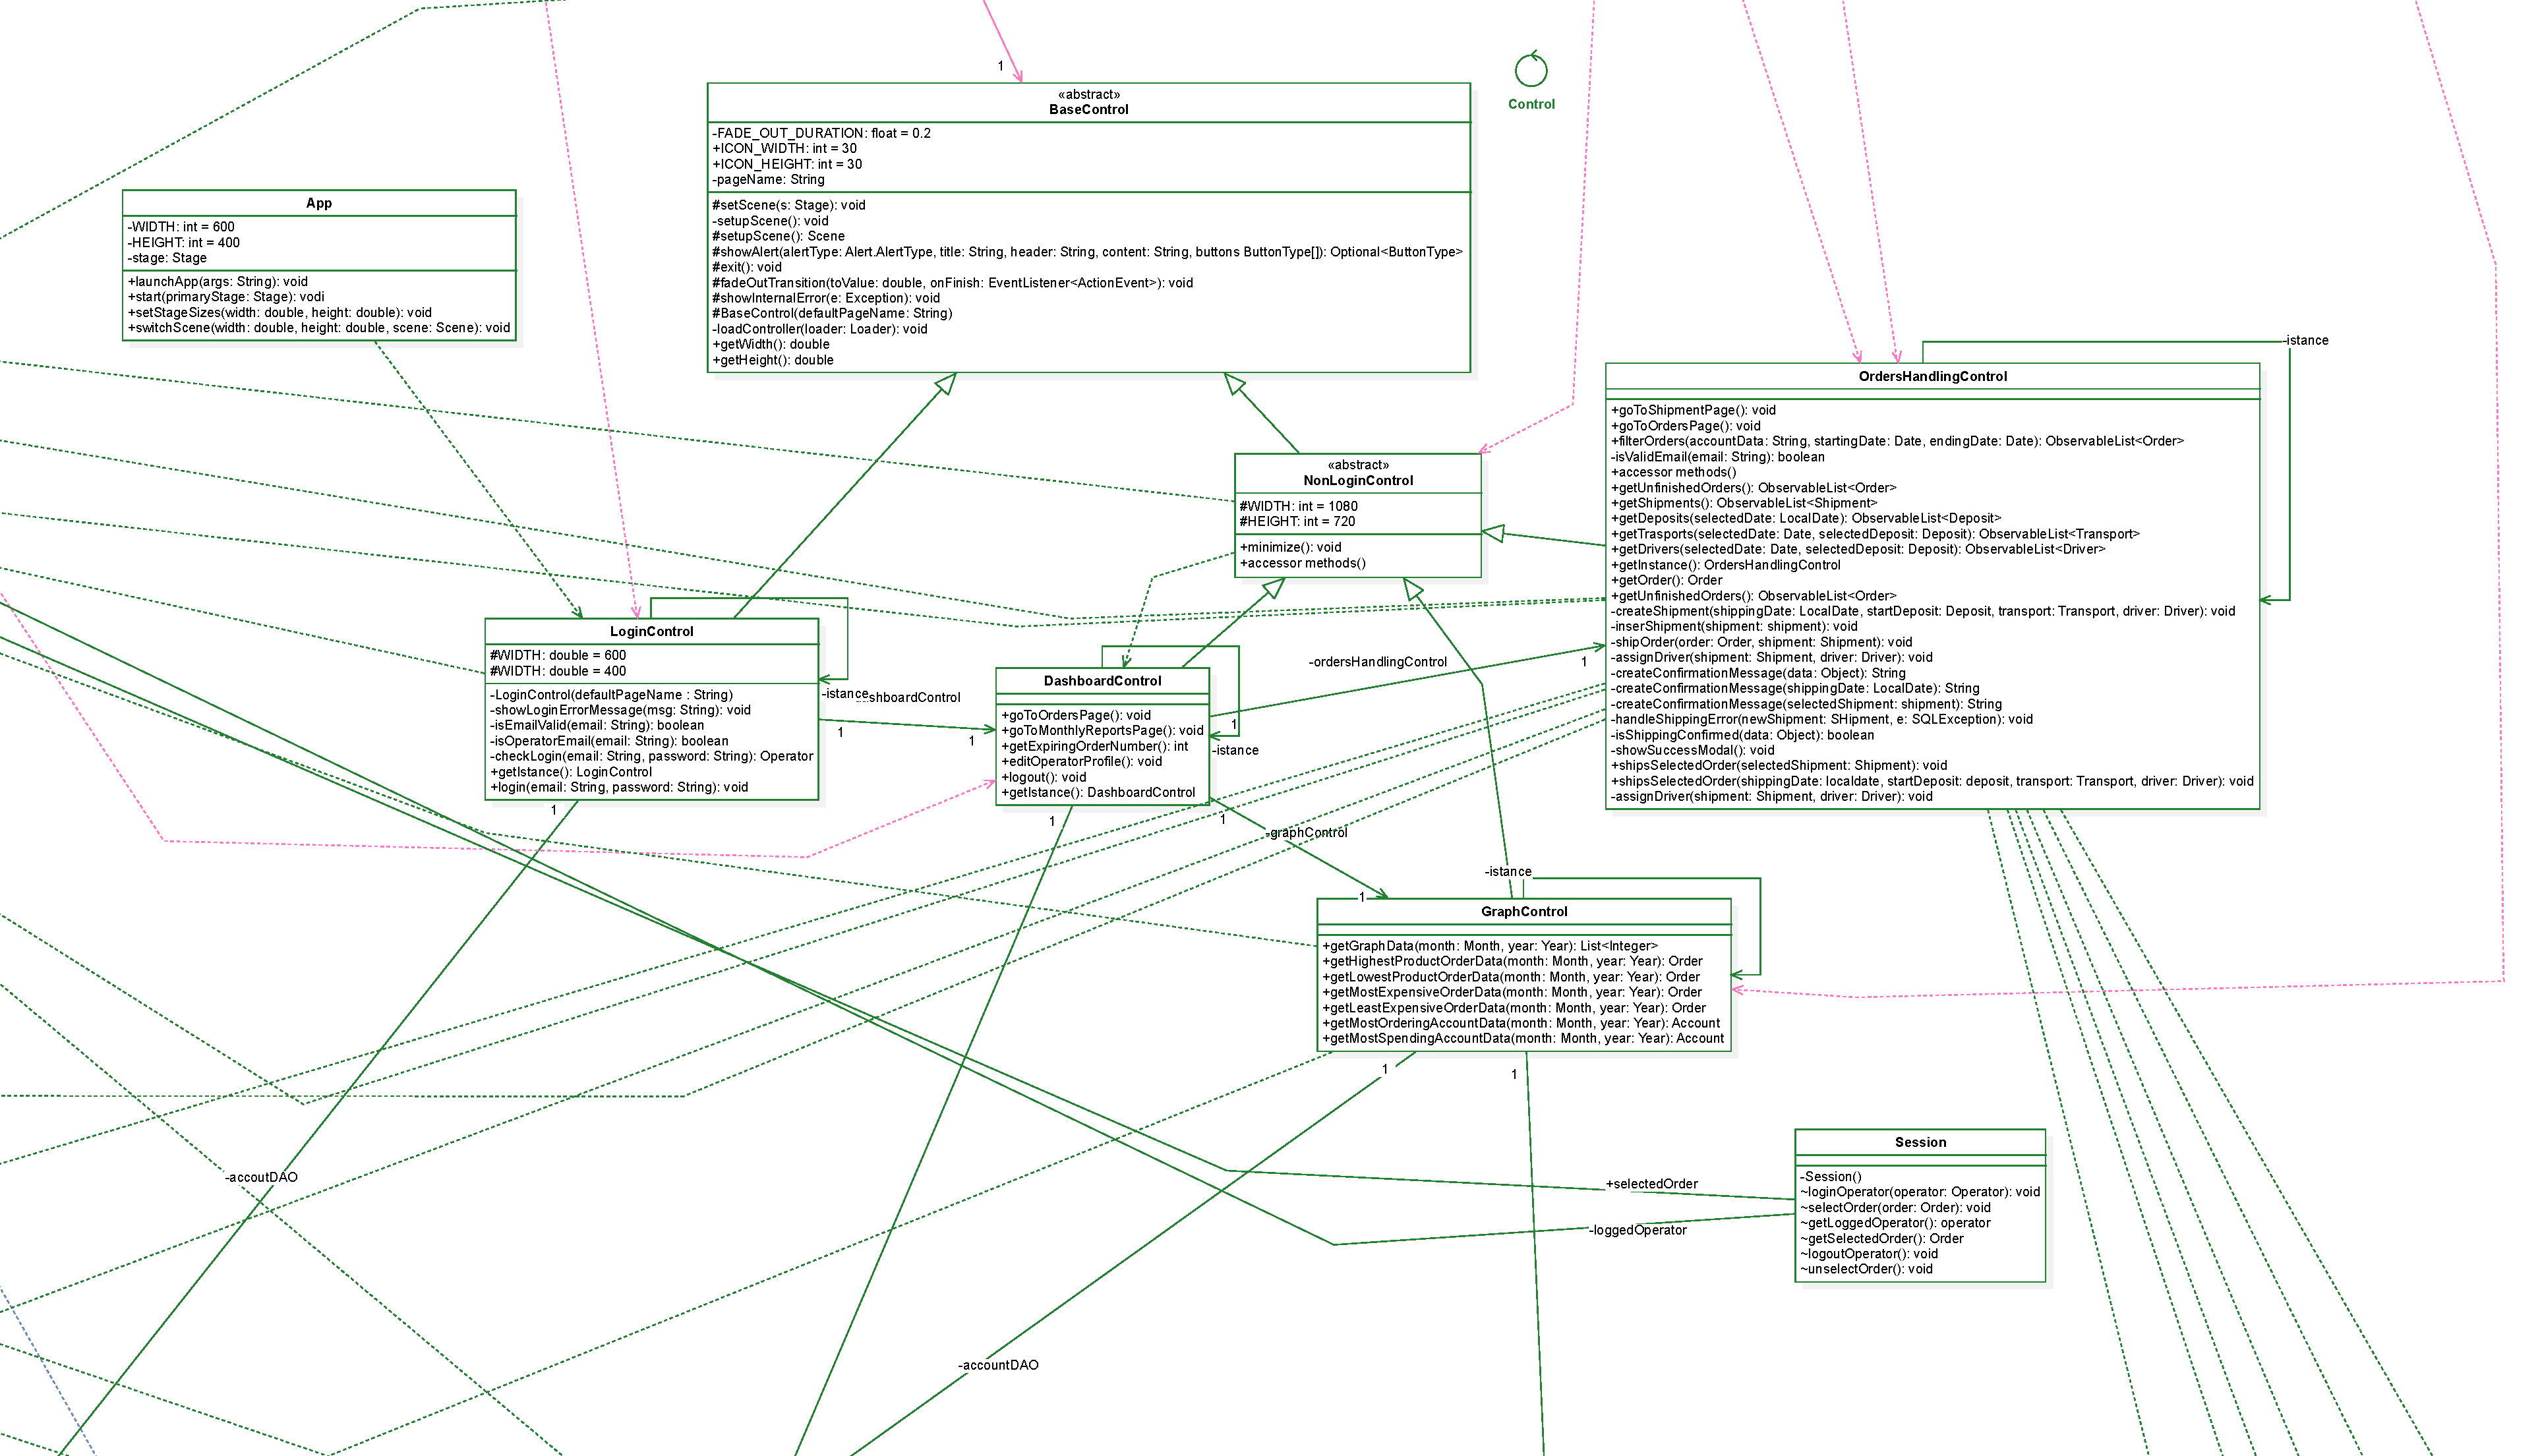
\includegraphics[width=\textwidth]{classDiagrams/controls}
  \caption{Class Diagram del package Control}
\end{figure}

\newpage

\subsection{Utils}

Inoltre, si è deciso di creare un package \textbf{Utils} contenente classi di utilità
per le altre componenti, ovvero classi che implementano metodi comuni a più classi
delle altre componenti, come ad esempio la gestione di \textbf{codifica e decodifica di dati
cifrati}, la gestione di \textbf{stringhe numeriche} o eccezioni personalizzate.

Tutte le classi di questo package sono \textbf{final}, in quanto non devono essere estese
e non istanziabili, avendo un costruttore privato, poiché, avendo esclusivamente 
\textbf{metodi static}, queste classi servono solo come supplier di metodi e non hanno
quindi necessità di uno stato interno.

In particolare, questo package contiene le classi:

\begin{itemize}
  \item \textbf{Base64ToImage} --- fornisce metodi per la conversione di stringhe Base64 in immagini
  \item \textbf{IterableInt} --- fornisce un \textbf{Iterator} per interi non superiormente limitato
  \item \textbf{LoadingScreen} --- fornisce metodi per la visualizzazione di uno schermo di caricamento
  \item \textbf{NumToStringFormatter} --- fornisce metodi per la formattazione di stringhe numeriche
  \item \textbf{SHA256} --- fornisce metodi per la codifica di stringhe in SHA-256
  \item \textbf{StaticResourcesLoadingException} --- eccezione personalizzata per la gestione di errori 
  di caricamento di risorse statiche come \textbf{file FXML e CSS}
  \item \textbf{UnimplementedMethodException} --- eccezione personalizzata per la gestione di errori
  di chiamata di metodi non implementati
\end{itemize}

\begin{figure}[H]
  \centering
  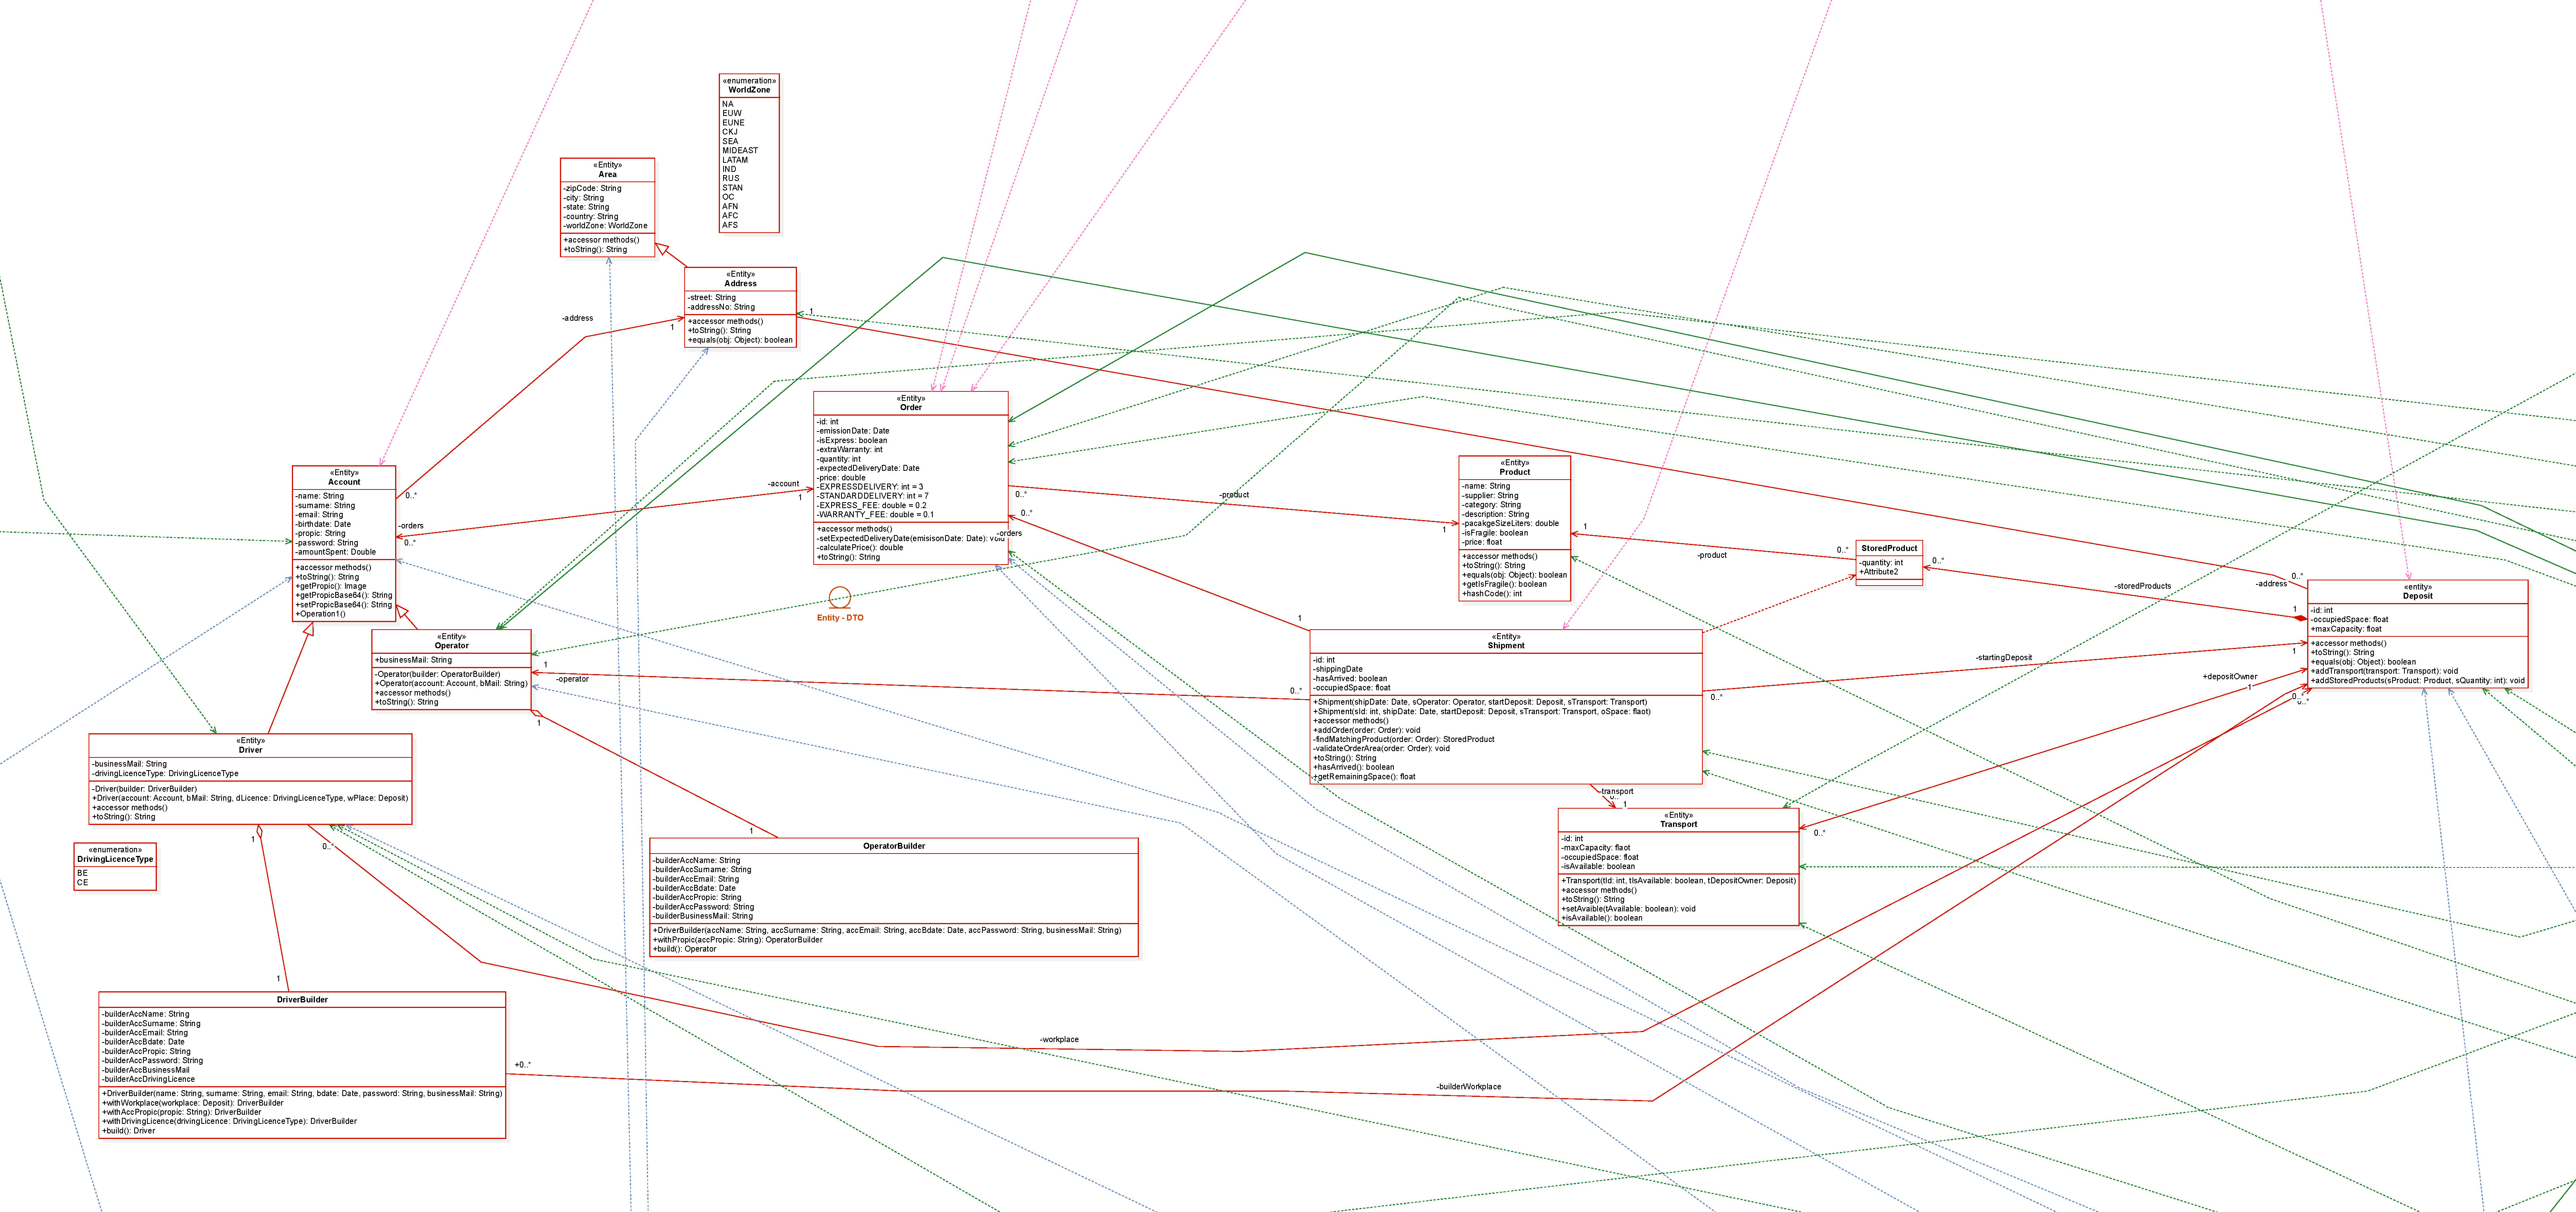
\includegraphics[width=\textwidth]{classDiagrams/utils}
  \caption{Class Diagram del package Utils}
\end{figure}

\newpage

\subsection{Class Diagram Completo}

\begin{figure}[H]
  \centering
  \includegraphics[width=\textwidth]{classDiagrams/full}
  \caption{Class Diagram Completo del Sistema}
\end{figure}